\documentclass[journal,10pt,twocolumn]{article}
\usepackage{graphicx}
\usepackage[margin=0.5in]{geometry}
\usepackage[cmex10]{amsmath}
\usepackage{array}
\usepackage{booktabs}
\usepackage{mathtools}
\title{\textbf{Optimization}}
\author{Lakshmi Kamakshi}
\date{September 2022}


\providecommand{\brak}[1]{\ensuremath{\left(#1\right)}}
\providecommand{\lbrak}[1]{\ensuremath{\left(#1\right.}}
\providecommand{\rbrak}[1]{\ensuremath{\left.#1\right)}}
\providecommand{\sbrak}[1]{\ensuremath{{}\left[#1\right]}}
\providecommand{\norm}[1]{\left\lVert#1\right\rVert}
\providecommand{\abs}[1]{\left\vert#1\right\vert}
\let\vec\mathbf
\newcommand{\myvec}[1]{\ensuremath{\begin{pmatrix}#1\end{pmatrix}}}
\newcommand{\mydet}[1]{\ensuremath{\begin{vmatrix}#1\end{vmatrix}}}

\begin{document}

\maketitle
\paragraph{\textit{Problem Statement} - To receive Grade 'A' in a course,one must obtain an average of 90 marks or more in 5 examinations. If sunita's marks in first four tests are 87,92,94and 95. find the minimum marks that sunita must obtain to get grade A in the course.} 
\section*{\large Solution}
Let x be the marks need to be scored by sunita in the fifth test.

\begin{figure}[h]
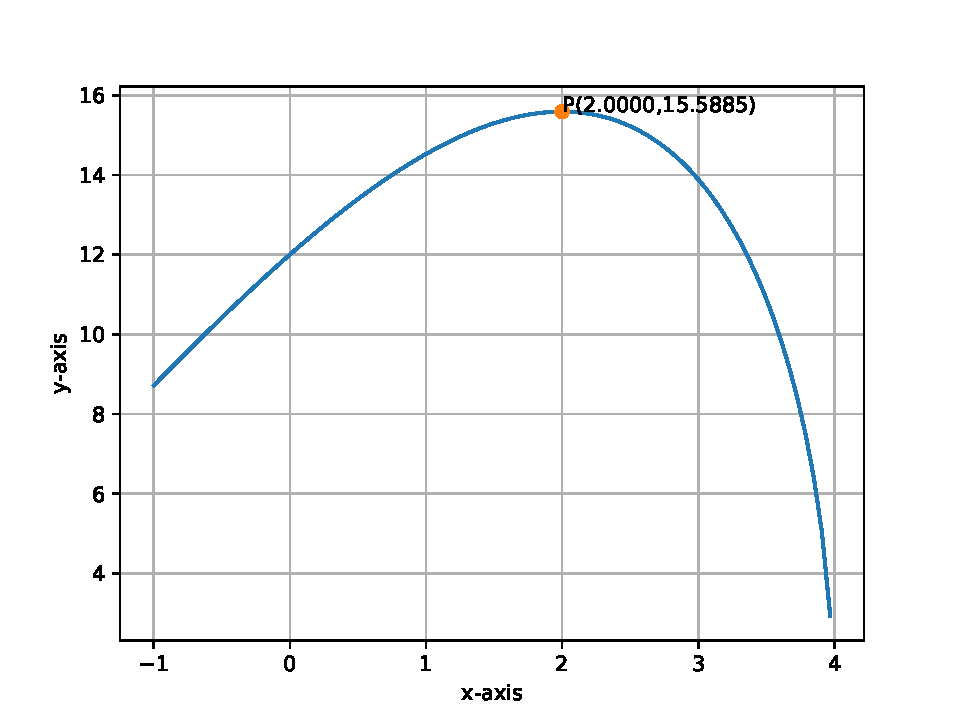
\includegraphics[width=1\columnwidth]{fig.pdf}
\end{figure}
\begin{align}
	P = \min_{x}x\\
	x + 368 \geq 450\\
	100 - x \geq 0 \\
\end{align}
which can be expressed in vector form as
\begin{align}
	P = \min_{\vec{x}}\vec{x}\\
	\myvec{1\\-1}\vec{x} + \myvec{368 \\ 100} \succeq \myvec{0\\0}
\end{align}
Solving using cvxpy, we get
\begin{align}
	P_{min} = 82\\
	\vec{x} = 82\\
\end{align}

\end{document}
